%%%%%%%%%%%%%%%%%%%%%%% file moduleX_template.tex %%%%%%%%%%%%%%%%%
%
%
% This is a template for creating your papers for the course KRW
% It is based on the standard Latex template for Springer publications
% but contains a suggestion for the structure and some content of the
% paper.
%
% Please adapt this document wherever needed.
%
% For more information about the required Latex Style check the document
% typeinst.pdf in the StyleFiles directory.
%
%%%%%%%%%%%%%%%%%%%%%%%%%%%%%%%%%%%%%%%%%%%%%%%%%%%%%%%%%%%%%%%%%%%%%%%%%


\documentclass[runningheads,a4paper]{../../StyleFiles/llncs}

\usepackage{url}
\usepackage{graphicx}
\usepackage{amssymb}


\newcommand{\keywords}[1]{\par\addvspace\baselineskip
\noindent\keywordname\enspace\ignorespaces#1}

\begin{document}

\mainmatter  % start of an individual contribution

% first the title is needed
\title{Ontology Matching Paper An ontology alignment over Amsterdam (Parking spots, events and activities)}

% a short form should be given in case it is too long for the running head
\titlerunning{Ontology Matching Paper}

% the name(s) of the author(s) follow(s) next
%
% NB: Chinese authors should write their first names(s) in front of
% their surnames. This ensures that the names appear correctly in
% the running heads and the author index.
%
\author{Alivanistos, Dimitris. \\ Baez, Selene. \\ Jemmett, Andrea.}
%
\authorrunning{Alivanistos, Dimitris. \\ Baez, Selene. \\ Jemmett, Andrea.}
% (feature abused for this document to repeat the title also on left hand pages)

% the affiliations are given next; don't give your e-mail address
% unless you accept that it will be published
\institute{\url{d.alivanistos@student.vu.nl} \and \url{s.baezsantamaria@student.vu.nl} \and \url{a.jemmett@student.vu.nl}}

\maketitle


\begin{abstract}
The abstract should summarize the contents of the paper and should
contain at least 70 and at most 150 words. It should be written using the
\emph{abstract} environment.
\end{abstract}


\section{Introduction}
%Introduce the sections that follow. What is the problem this paper addresses? What is the core contribution of this paper, and why is that interesting? What method did you develop and implement? What is the research question or hypothesis this paper answers? How did you answer this question or validate your approach (empirically, analytically). You might want to give a brief (qualitative) sketch of the results. 
In this paper we continue the work related for creating an application for finding Handicap Parking Spots close to Event Venues in Amsterdam. In the previous paper, we improved on the ontology to comply with the Five Star model and linked it to other existing ontologies. In this paper, we continue the work by matching and aligning the ontology to other subject-related ontologies. 

In general, the problem of matching ontologies has been studied before by Semantic Web researchers. As Shvaiko et al. state, the problem of heterogeneity is still a challenge to be solved since ambiguity in meanings and interpretations prevent us from finding equivalences in same domain ontologies \cite{shvaiko2013ontology}. Ontology matching and alignment allow to merge, translate, and extend ontologies, finding correspondences in entities, properties and instances. The Ontology Alignment Evaluation Initiative is an annual international competition that serves as an evaluation for state of the art alignment tools. 

With that in mind, in this paper we select relevant vocabularies from the pool of Amsterdam related ontologies in our class. After some comparison we selected Group 10 -an ontology for cultural activities-, Group 13 -an ontology about safety for tourists using statistical area information-, and Group 15 -an ontology for general activity finding.

In the following sections we first revise existing tools for matching and aligning ontologies. Then we select and apply tools for matching and aligning our ontologies to the aforementioned ones, experimenting with different comparators. We continue to evaluate such algorithms and discuss the results. Finally, we conclude by summarizing the findings of the alignment to different ontologies.

\section{Related Work}
\label{related_work}
%Give here an overview over related matching methods and how they related to your own solution. Cite papers that might have inspired your approach. Sometimes it makes sense to have this section immediately after the introduction.
In order to match our ontology to others, we did research about state of the art matching and alignment tools. \cite{adaptiveInformation_2014} is a comprehensive list of the top 50 tools, separating active from inactive tools. Additionally, we looked at some of the tools revised by Euzenat et Al \cite{euzenat2007ontology}. Furthermore, we looked at the participants from the most recent OAEI.

In the following we list the most relevant tools.

\begin{enumerate}
	\item \textbf{OLA \cite{euzenat2004ontology}:} Developed in 2004, the OWL Lite Alignment (OLA) is a tool for automatic matching of ontologies that implements the OLA algorithm designed in collaboration by the DIRO, University of Montréal and INRIA Rhône Alpes. It participated in OEIA 2005 \cite{euzenat2005ola} and 2007 \cite{djoufak2007ola} and increased its own results from 0.80 to 0.89 in Precision, and 0.74 to 0.87 in Recall. At the time, it was one of the pioneers of ontology matching, yet the project was abandoned and it is nowadays outdated.
	\item \textbf{S-Match \cite{giunchiglia2004s}:} S-Match is a semantic matching tool that is suitable for many applications. However, it is not specific for ontology matching and it has not participated in the latest OAEI.
	\item \textbf{MapONTO \cite{an2004refining}:} MapOnto, just as S-Match, is a general purpose semantic matcher. It is an initiative from the University of Toronto and it is implemented as a plug-in for Protege. At first sight, this option seemed promising, however the latest release is only compatible with obsolete versions of Protege. 
	%\item \textbf{WordNet:Similarity \cite{pedersen2004wordnet}:} Semantic 
	\item \textbf{AML \cite{faria2013agreementmakerlight}:} The Agreement
	Maker Light (AML) is the improved version of the original Agreement Maker. It is a simple, user-friendly application for matching ontologies which also provides visualization and evaluation of the alignment. Further details will be discussed in Section \ref{Ontology_Matching}.
\end{enumerate}

\section{Methods, Algorithms and Implementation}
% Introduce your method, i.e. the overall approach taken and the general idea, the\bibliography{paper} algorithms in general, maybe in pseudo-code and give a quick overview over the technical implementations (not too much details).
With the results from Section \ref{related_work}, we selected AML for ontology matching and SILK for ontology alignment. The similarity measures applied for both of the above were studied from \cite{sun2015comparative}.

% Maybe you want to separate this part into subsections for your two systems
\subsection{Ontology Matching}
\label{Ontology_Matching}
Looking at the most recent OAEI results, we decided to use one of the best candidates in the OAEI of 2014: AML. This tool performed the best for lightweight ontologies, as measured in terms of F-measure \footnote{The F-measure is the harmonic mean of Precision and Recall.}. AML exceeded our expectations with regards to run time results, comprehensive user interface and integrated evaluation mechanism. The procedure can be fully or semi automatic, with the user being presented to a fully customizable matching. A lexical matching is always performed as default, followed by other metrics the user can choose from, ranging from structure to content based and others. Furthermore, AML provides with visualizations for the matches as shown in Figure \ref{fig:single_match}, \ref{fig:multiple_match} and \ref{fig:incorrect_match}.
%examples with pictures, String Matcher, Word matcher, Property matcher, Cardinality matcher and background knowledge matcher.

\begin{figure}[h]\centering
	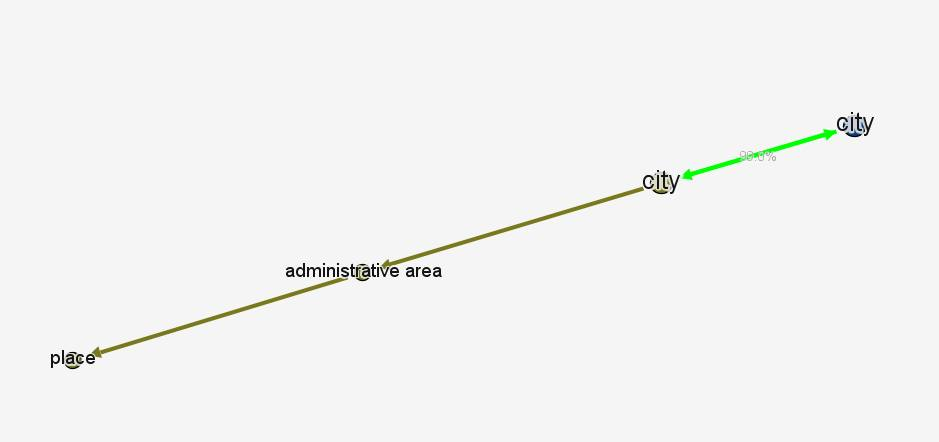
\includegraphics[width=.8\textwidth]{img/match_city.png}
	\caption{Visual representation of a single correct match in AML.}
	\label{fig:single_match}
%\end{figure}
%\begin{figure}[h] \centering
	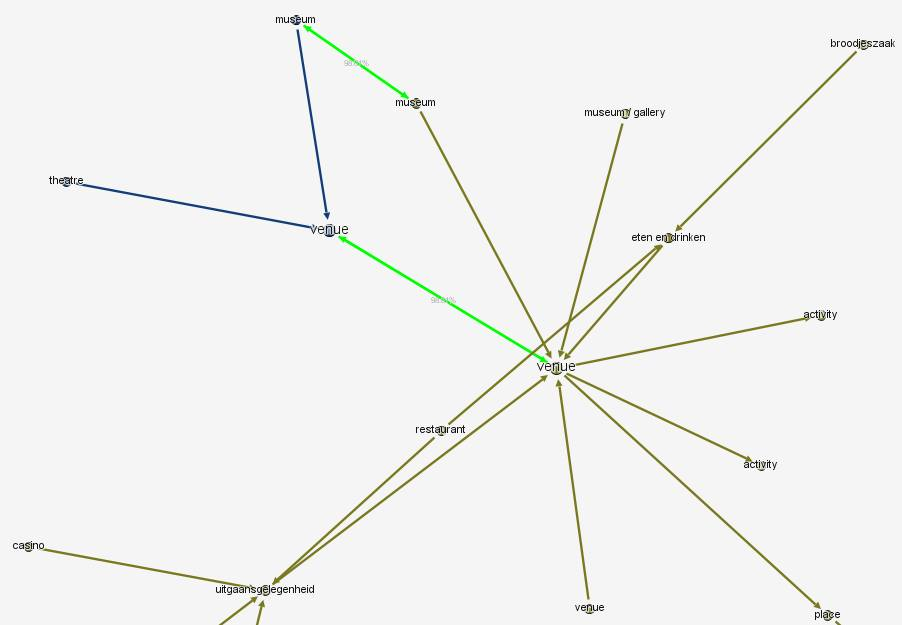
\includegraphics[width=.8\textwidth]{img/match_combo.png}
	\caption{Visual representation of multiple correct matches in AML.}
	\label{fig:multiple_match}
%\end{figure}
%\begin{figure}[h] \centering
	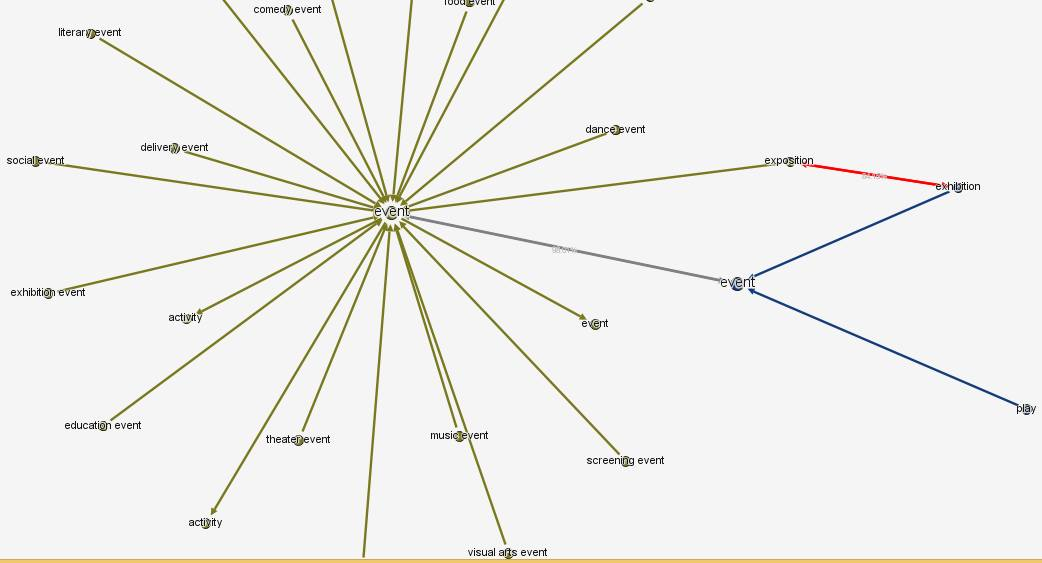
\includegraphics[width=.8\textwidth]{img/conflict_exhibition_exposition.png}
	\caption{Visual representation of an incorrect match in AML.}
	\label{fig:incorrect_match}
\end{figure}

The power of AML is shown as its ability to combine different types of matchers, in a hierarchical or concurrent manner. Our method was to test each matcher separately in order to study the results obtained, while in a later stage we experimented with different combination of matching (i.e. Word matching, String matching and Structural matching). Furthermore, AML also allows the user to customize the settings of the matchers. For example, regarding String matcher it gives the option to choose between four different similarity measures: iSub, Levenstein, Jaro-Winkler and Q-gram, as described by Sun et al. \cite{sun2015comparative}.

\subsection{Data Linkage}
In this section the developed Data Linkage system is presented. It interlinks our dataset with the previously mentioned datasets from groups 10, 13 and 15. We decided to implement the linking workflow and procedures using the \textit{Silk framework}\footnote{\url{http://silkframework.org/}} which captions itself as ``The Linked Data Integration Framework''. Silk is an open source project for integrating heterogeneous data sources. Its use cases include generating links between Linked Data sources, which is exactly within our needs. Moreover Silk provides the user with a nice and friendly Web-based GUI and a visual editor for linkage rules.

To link two Linked Datasets using Silk first we need to define their sources, e.g. using a SPARQL endpoint or uploading an RDF dump. Then it is possible to create linkage rules by applying four different kind of operations:
\begin{enumerate}
	\item path-like queries to retrieve values;
	\item transformations over those values (e.g. to-lowercase, tokenization);
	\item comparators over values (e.g. Levenshtein distance, Jaccard
		coefficient, equality);
	\item aggregators over comparators output (e.g. average, minimum, maximum).
\end{enumerate}
It is also possible to specify a threshold for the comparator's output score, its weight when computing an aggregation for it or whether it is required that a value exists for that block\footnote{We say block because Silk uses a visual editor with block-shaped functionalities.}.

In the following sections we show how we implemented a Data Linking system to
link our dataset with three other datasets created by peers following our same
class\footnote{Knowledge Representation on the Web at VU Amsterdam, 2015/2016}.
Moreover we tried to look-up the Linked Open Data cloud searching for similar
datasets that we could link to ours. We used
LOTUS\footnote{\url{http://lotus.lodlaundromat.org/}}, a tool from the LOD
Laundromat suite\footnote{\url{http://lodlaundromat.org/}}\cite{beek2014lod}
that allows to search the LOD cloud for statements based on some query
parameters. Unfortunately we were not able to find interesting datasets there.

\subsubsection{Linking Group 10: Cultural Ontology}
This dataset has a domain similar to ours so the linking procedure
is trivial and is reduced to a check on the \texttt{rdfs:label} combined with some other property. An example of a Silk linkage rule that matches Events is shown in Figure \ref{fig:link_event_g10}. In this case the match is checked against \texttt{rdfs:label} and \texttt{dc:title}. With this rule we are able to create 15 links over 239 source and 479 target event entities.

\begin{figure}[h]
	\centering
	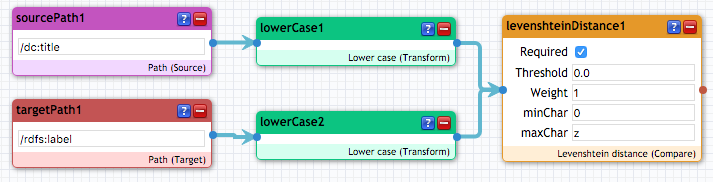
\includegraphics[width=1\textwidth]{img/link_event_g10.png}
	\caption{Silk linkage rules for events in group 10's dataset.}
	\label{fig:link_event_g10}
\end{figure}

\subsubsection{Linking Group 13: Tourist safety Ontology}
In spite having a different domain, this dataset can still be linked to ours for what concerns events and locations / venues. Indeed the overlap between events in this dataset and ours is large. We are able to match a larger proportion of entities by using a linkage rule similar to that shown in Figure\ref{fig:link_event_g10} but using \texttt{rdfs:label} for both data sources. Using this linkage rule we are able to link 45 events and locations between the two datasets.

\subsubsection{Linking Group 15: Activity finding Ontology}
\label{link_g15}
This time the linkage rule for events is less trivial and immediate than that for the previous two datasets. As such, it involves the use of more properties and an aggregator as shown in Figure \ref{fig:link_event_g15}. With this linkage rule we are able to link 84 activities / events.

\begin{figure}[h]
	\centering
	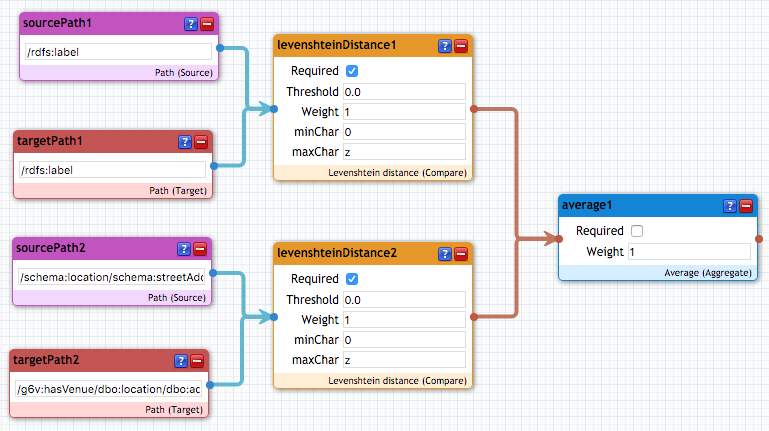
\includegraphics[width=1\textwidth]{img/link_event_g15.png}
	\caption{Silk linkage rule for events in the Activity Finding Dataset.
		\texttt{sourcePath2} contains
		\texttt{/schema:location/schema:streetAddress} while
		\texttt{targetPath2} contains
		\texttt{/g6v:hasVenue/dbo:location/dbo:address}.}
	\label{fig:link_event_g15}
\end{figure}

\section{Validation and Experiments}
% In a scientific paper you want to show that your choice of method and algorithms was the right choice. So, this could be a place where you make claims or ask concrete and explicit research questions (e.g. with respect to runtime and/or precision/recall.
We conducted a variety of experiments regarding the matching of our ontology (consisting of 16 classes, 24 properties and 6 individuals) to others. This was made possible by how customizable AML is.

We tried different similarity measures for String and Word matching as well as different filters regarding cardinality and coherence. Results mostly remained unchanged, and we believe this is due to the limited size and complexity of the ontologies presented. However, it is worth mentioning that strict, permissive and hybrid cardinality filters had a significant impact on the resulting alignment. For example, with regards to the matching with group 15, hybrid or permissive filters matched our Event class with 3 different classes of their ontology while with strict filter, we got a single match. 

AML also has the ability to evaluate a certain match with respect to a reference match. This gives the option for the end user to manually force or evaluate the match and thus supervise and validate the final match. As so, the user can match classes or properties by hand and use the corrected match as reference for future matchings.

Hereby we report the results of evaluating the automatic matching procedure, as performed by AML, with the human validated alignment for the three selected ontologies. Basic characteristics for the ontologies, as well as a visualization of the matching in AML are given for each case.

\subsection{Group 10: Cultural Ontology}
This ontology consists of 11 classes, 23 properties, 1 individual. Our ontology matches to their main entities of Events and Venues. A visualization of the matching is presented in Figure \ref{fig:match_g10}.

\begin{figure}[h]\centering
	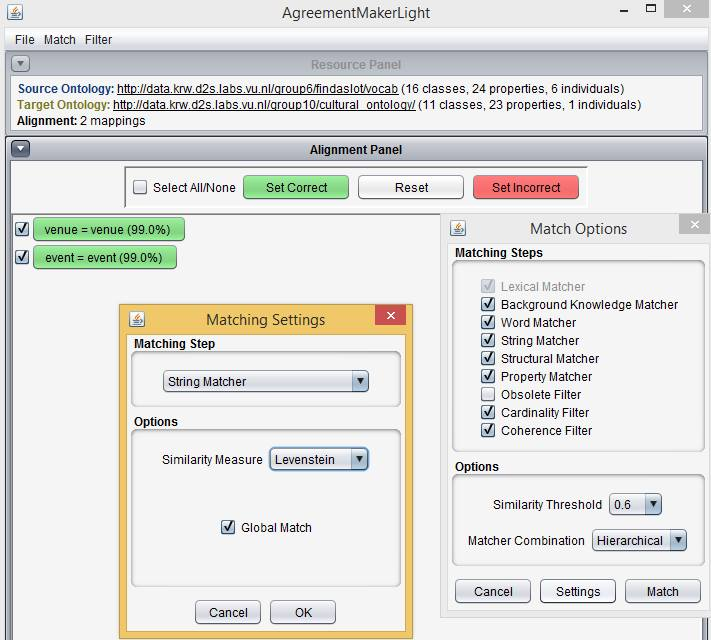
\includegraphics[width=.7\textwidth]{img/match_g10.png}
	\caption{Matching to group 10}
	\label{fig:match_g10}
\end{figure}

AML found two mappings leading to the following evaluation metrics:

\begin{center}
	\begin{tabular}{| c | c | c |}
		\hline
		\textbf{Precision} & \textbf{Recall} & \textbf{F-measure} \\ \hline
		100\% & 100\% & 100\% \\ \hline
	\end{tabular}
\end{center}

\subsection{Group 13: Tourist safety Ontology}
This ontology consists of 16 classes, 20 properties, 973 individuals. We matched Events, Location, City as well as Start and End date. The entity for Country was mistakenly matched to the Area entity. A visualization of the matching is presented in Figure \ref{fig:match_g13}.

\begin{figure}[h]\centering
	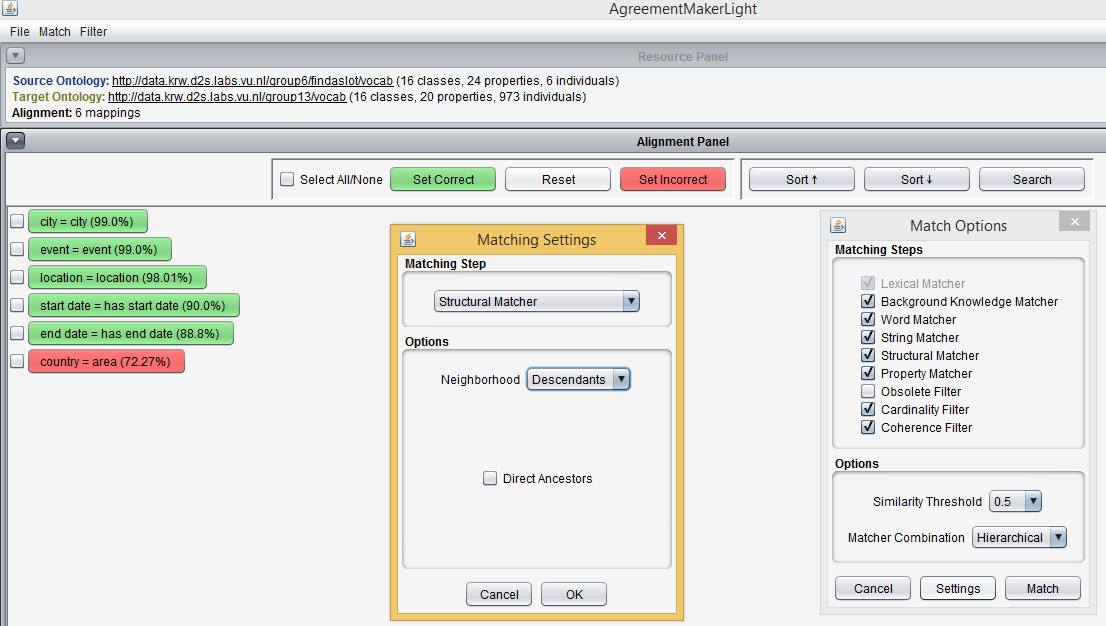
\includegraphics[width=.7\textwidth]{img/match_g13.png}
	\caption{Matching to group 13}
	\label{fig:match_g13}
\end{figure}

AML found 6 mappings, leading to the following evaluation metrics: 

\begin{center}
	\begin{tabular}{| c | c | c |}
		\hline
		\textbf{Precision} & \textbf{Recall} & \textbf{F-measure} \\ \hline
		83.3\% & 100\% & 90.9\% \\ \hline
	\end{tabular}
\end{center}

\subsection{Group 15: Activity finding Ontology}
In this case, the target ontology consists of 66 classes, 599 properties and 57 individuals. This is, by far, a larger ontology than ours and the previous examined ontologies. A visualization of the matching is presented in Figure \ref{fig:match_g15}.

\begin{figure}[h]\centering
	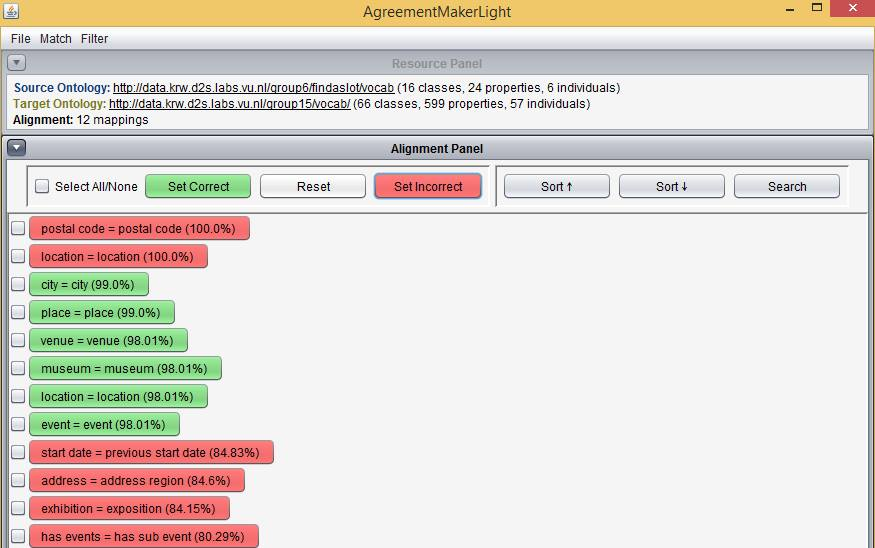
\includegraphics[width=.7\textwidth]{img/match_g15.png}
	\caption{Matching to group 15}
	\label{fig:match_g15}
\end{figure}

AML found 12 mappings, six correct versus six incorrect matchings, leading to the following evaluation metrics: 

\begin{center}
	\begin{tabular}{| c | c | c |}
		\hline
		\textbf{Precision} & \textbf{Recall} & \textbf{F-measure} \\ \hline
		54.5\% & 46.2\% & 50.0\% \\ \hline
	\end{tabular}
\end{center}


\section{Results and Discussion}
% Give here details about the most important results of your experiments. Use tables and figures, but focus on the interesting and important results. Make sure you describe in the text what the reviewers should see, explain what the reader sees in the tables and point to the interesting findings. Be explicit about your research question and hypothesis, and discuss they might be true, or false. 
From the previous section we observe that the ontology for group 13 has the highest number of matches (six) with the least number of mismatches (one). Yet, the matching only works for one of our three basic entities (Events, Venues and Parking Spots). 

At the same time, the ontology for group 15 produces the same number of matches (six) but it has a high number of mismatches as well (six). Most of the mismatches come from Properties, since this particular ontology has a high degree of customizable properties with ambiguous names. 

However, regardless of having the same number of matches, the ontology for group 15 led to a higher number of links to our ontology than for group 13. This is due to the higher overlap in instances that allows for a closer alignment.

A second observation is one made for the performance of matching with group 10. Conflicting with our initial hypothesis, the matching with the group 10's ontology did not perform as well as expected. Intuitively, we believed that our ontology should have had more matches with this group, since they model the same datasets as we do. However, they model characteristics of events as Entities (such as Image, Description and Time Period), while we do it as Properties. To the best of our knowledge, AML cannot match entities to properties. This discovery raises more serious questions since the limitations of matching are evident when design decisions like the ones in this case rigidly prevent proper matching and alignment.

A third observation regards a different problem occurring in the case of the matching to the ontology of group 15. In this case, we found overmatching since their ontology has duplicate classes for Museum, Venue and Event. Therefore, several metrics failed to distinguish the duplicate match resulting in AML outputting misleading results. This matching required the most amount of work regarding experimenting and tuning of matching, as well as alignment with SILK as mentioned in Section \ref{link_g15}. As stated before, details as fine as the specific type of cardinality filter greatly affected the end result. 


\section{Conclusion}
%Here you summarize the preceding sections, describe the lessons learnt and discuss future work.
In this paper we matched our ontology for finding Handicap Parking Spots in Amsterdam to other ontologies related to entertainment in Amsterdam. We found that the match with the highest confidence corresponds to Group 10, but the match with highest overlap corresponds to Group 15 closely followed by Group 13.

From the experiments performed we learned that great amount of work is invested in applying the correct similarity measures. Furthermore, our experience is backed up by the findings described in Section \ref{related_work}. As we see, Ontology matching is a growing field, that comes up with new promising tools every year. Yet, follow up is not consistent and a robust solution for automatic, or semi-automatic ontology matching has yet to be developed.



\bibliographystyle{plain}
\bibliography{mybib}

\end{document}
